% !TeX root = ../__ylc_main.tex

\chapter{学生思维能力建模方法}

\section{学生表述解题过程的特点}

在解决问题的过程中,人类学生对于解题过程思路的理解与机器对其的理解往往存在差距。学生在解题过程中,会通过一系列的思维活动理解问题、选择解题方法、实施解题过程以及验证结果。这一过程涉及到多种认知活动,包括信息提取、推理、计算和验证等。然而,学生在表述解题过程时,往往会由于多种因素的影响,导致其表述存在一定的不确定性和复杂性。这使得机器在理解学生的解题过程时面临一定的挑战。为了更好地理解学生的解题过程,需要对学生表述解题过程的特点进行详细分析。

对于本研究关注的高中数学解答题,学生在完成数学解题时,通常会有一套较为固定的思维路径和方法。一般来说,学生在解题过程中会经历以下几个阶段:

\begin{itemize}
    \item 理解问题:学生首先需要对题目进行全面的理解,明确题目所要求的目标和已知条件。这一阶段学生会通过阅读、分析题目并提取关键信息来形成对问题的初步认识。
    \item 选择方法:在明确问题之后,学生需要选择适当的解题方法或策略,明确解题路径。
    \item 实施解题过程:学生根据所选的解题方法一步步进行操作,这一过程中通常会涉及到一系列的计算和推理。就逻辑性较强的数学学科的推导而言,对于每一步推理,往往遵循着这样的模式:基于某些已知条件,运用某个特定的数学规律,得到某个新的结论。
\end{itemize}

对于解题过程中每一步的推理,此处进行进一步明确以方便下文的讨论。在解题的初始状态,学生在读题并理解后,脑中会有一个信息的集合,这个集合包括了所有题给条件信息,以及学生记忆中所有与本题相关的知识点和方法。随后的每一步推理,可以认为是在这个信息集合的基础上,运用合适的数学方法,基于已有信息集合的一个子集,通过计算或推导得到一个新的结论,这个新的结论会被加入到信息集合中。这个过程会一直持续到学生得到最终的解答。在这个过程中,学生的思维活动是一个动态的、逐步推理的过程,每一步推理都是基于已有的信息(可能包含先前推出的结果),不断更新本题的“内存空间”。

然而,学生在表述其解题过程时,往往存在一些特点,这些特点使得机器理解学生的解题过程变得复杂。首先,由于人与机器感知方式的差异,二者所能收集到的信息存在差异。其次,人类的记忆是一个动态的、非格式化的、可能出现模糊和错误的信息载体。学生在表述解题过程时,可能会使用不同的语言表达方式和数学符号,不同学生的语言习惯、用词偏好以及对符号的使用存在差异;同时,学生描述某一步推理时的表述方式可能是比较高级的、抽象的(例如“通过观察可以得知”),也可能是详细的、底层的、具体的(例如“根据勾股定理和上一步求出的两条边的长度,可以得到……”)。学生在解题时口头描述的解题过程,是非结构化的语言数据,相较于结构化的书面解答,口头描述包含更多的噪音和不确定性,机器需要具备更强的自然语言处理能力来提取有用信息。此外,学生在解题过程中可能会出现思维跳跃、错误和修正等现象,也有可能出现解题中途发现遇到困难,换一种方法从头开始的情况,这些现象使得学生的解题过程不是一个线性的、单向的过程,而是一个动态的、多变的过程。

这些因素都增加了机器解析人类学生解题过程的难度。比如在知识和已有信息的储存记忆方面,机器如果使用某种数据库来储存高中数学知识的话,一定是有统一的数据结构的、清晰的、无误差的,这与学生记忆所可能出现的模糊性相反。考虑到学生表述解答过程中的多样性,在处理学生的表述时往往面临着机器能力理解不足、从机器规则难以获得预期效果等问题,传统方法也缺乏将学生表述的的非结构化步骤转化为结构化机器数据的能力。

为了弥合机器与人类学生对于做题推理步骤理解的差距,本研究认为需要提出新的有效方法来设计系统,从而对学生的解题过程进行有效的建模。机器需要具备较强的自然语言处理能力,能够解析学生的语言表述和数学符号,并将其转化为可处理的逻辑结构。此外,机器还需要能够处理多步推理和动态修改的复杂性,确保对学生解题思路的准确跟踪和建模。最重要的是,机器需要具备可靠的错误识别和分析能力,能够在学生犯错时识别出错误所在,并进行相应的错因分析,进而实现个性化辅导。

为了解决上述问题,本研究计划基于大语言模型(LLM)来进行学生思维能力的建模。为了探究学生在解题过程中会如何表述自己的思路,本研究先开展了一次预实验,通过让学生口头描述自己的解题过程,收集学生解题过程中的语音、视频和笔迹数据,然后对学生的这些数据进行分析,从中总结学生表述解题的过程中有哪些特点,对解决上述机器理解人类做题推理过程的理解这一挑战有何启示,进而指导后续的系统设计。

\section{实验探究解题过程表述特点}

本研究在着手进行系统设计之前先进行了一次预实验,在实验室环境中请参与者解答高考数学题,通过手写板和智能平板来收集解题过程的笔迹、视频和音频信息,并由人类专家实时观察解题过程。本次实验的详细设计如下所述。

\subsection{实验设计}
在题目选择上,我们选择了三道高考数学题,分别涉及到数列、立体几何和导数的知识,题目难度适中,既有一定的思维含量、需要一定的高中数学知识和技能来求解、可能会有多种解法,难度又没有很高以至于令大多数学生感到无从下手,适合用于本次实验。这三道题目分别是:

\begin{quote}
    \begin{description}
        \item[题目一] 记 $S_n$ 为数列 $\left\{a_n\right\}$ 的前 $n$ 项和, 设甲: $\left\{a_n\right\}$ 为等差数列:乙: $\left\{\frac{S_n}{n}\right\}$ 为等差数列. 则

        A. 甲是乙的充分条件但不是必要条件

        B. 甲是乙的必要条件但不是充分条件

        C. 甲是乙的充要条件

        D. 甲既不是乙的充分条件也不是乙的必要条件

        \item[题目二] 已知圆锥的顶点为 $P$, 底面圆心为 $O, A B$ 为底面直径, $\angle A P B=120^{\circ}, P A=2$, 点 $C$ 在底面圆周上, 且二面角 $P-A C-O$ 为 $45^{\circ}$(图片参见\ref{fig:problem_2_fig}), 则

        A. 该圆雉的体积为 $\pi$

        B. 该圆雉的侧面积为 $4 \sqrt{3} \pi$

        C. $A C=2 \sqrt{2}$

        D. $\triangle P A C$ 的面积为 $\sqrt{3}$

        \item[题目三] 已知函数 $f(x)=a\left(\mathrm{e}^x+a\right)-x$.

        (1) 讨论 $f(x)$ 的单调性:

        (2)证明:当 $a>0$ 时, $f(x)>2 \ln a+\frac{3}{2}$.
    \end{description}
\end{quote}

\begin{figure}
    \centering
    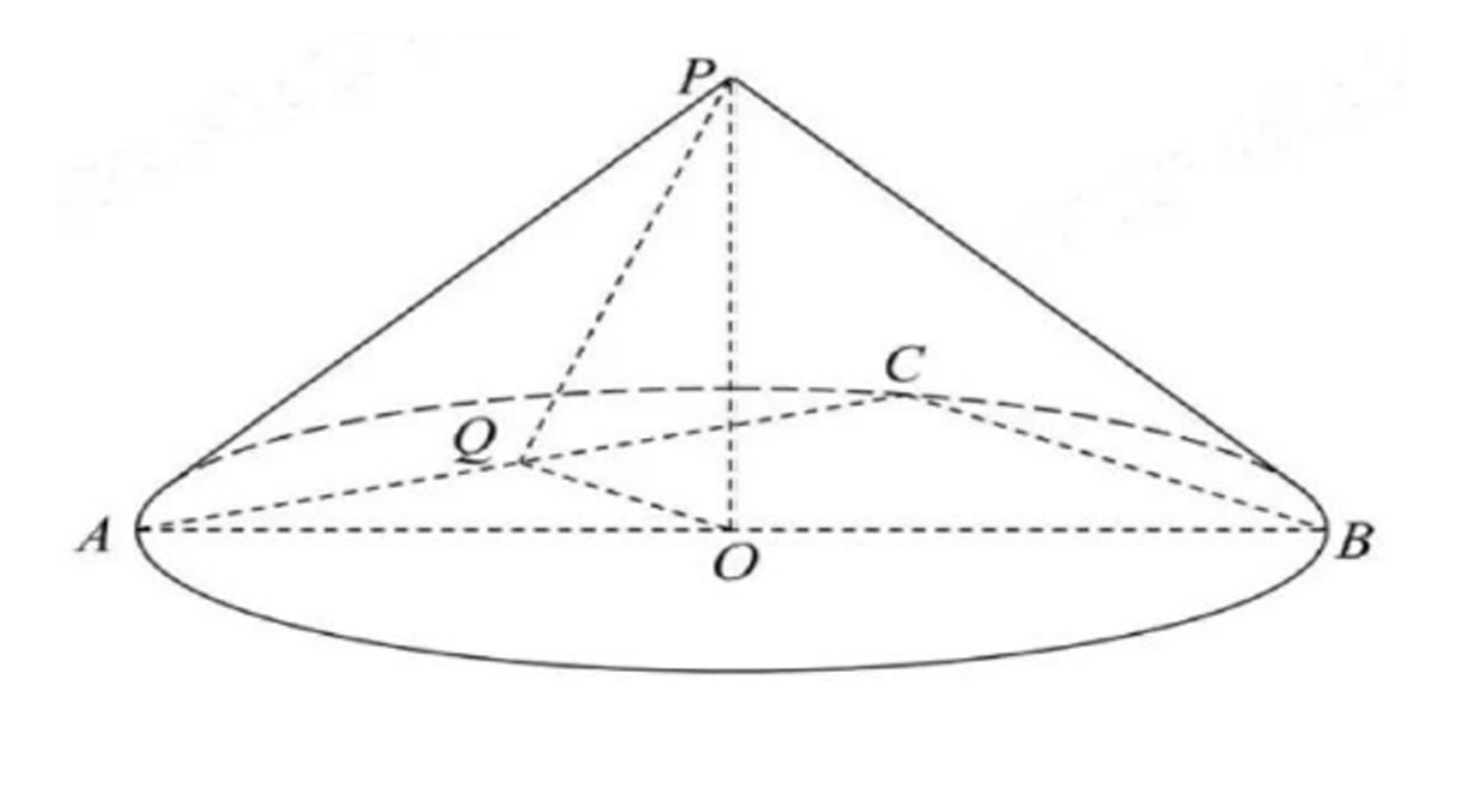
\includegraphics[width=0.5\linewidth]{problem_2_fig.png}
    \caption{预实验中题目二的配图}
    \label{fig:problem_2_fig}
\end{figure}

我们在校内招募了8名本科生作为被试参与了本次实验,这8位被试中有3位女生,5位男生;他们来自不同的院系,年龄从19岁到22岁不等。每个参与者完成实验(求解完三道数学题)的用时一般在30分钟到50分钟之间。我们给每位参与者提供实验补偿。在实验结束后,实验人员可能会对参与者的解题过程进行一定的访谈,以了解参与者在解题过程中的思考和策略中表达较模糊的部分。

实验使用一块数位板来采集被试解题过程的手写笔迹数据,使用安卓平板电脑来收集视频和音频数据。我们在安卓平台开发了一个应用程序,用来连接数位板、展示题目,以及采集并记录上述数据。实验所需的硬件设施如图\ref{fig:experiment_setup}所示,实验器材的详情会在后续章节进行详细说明。

\begin{figure}
    \centering
    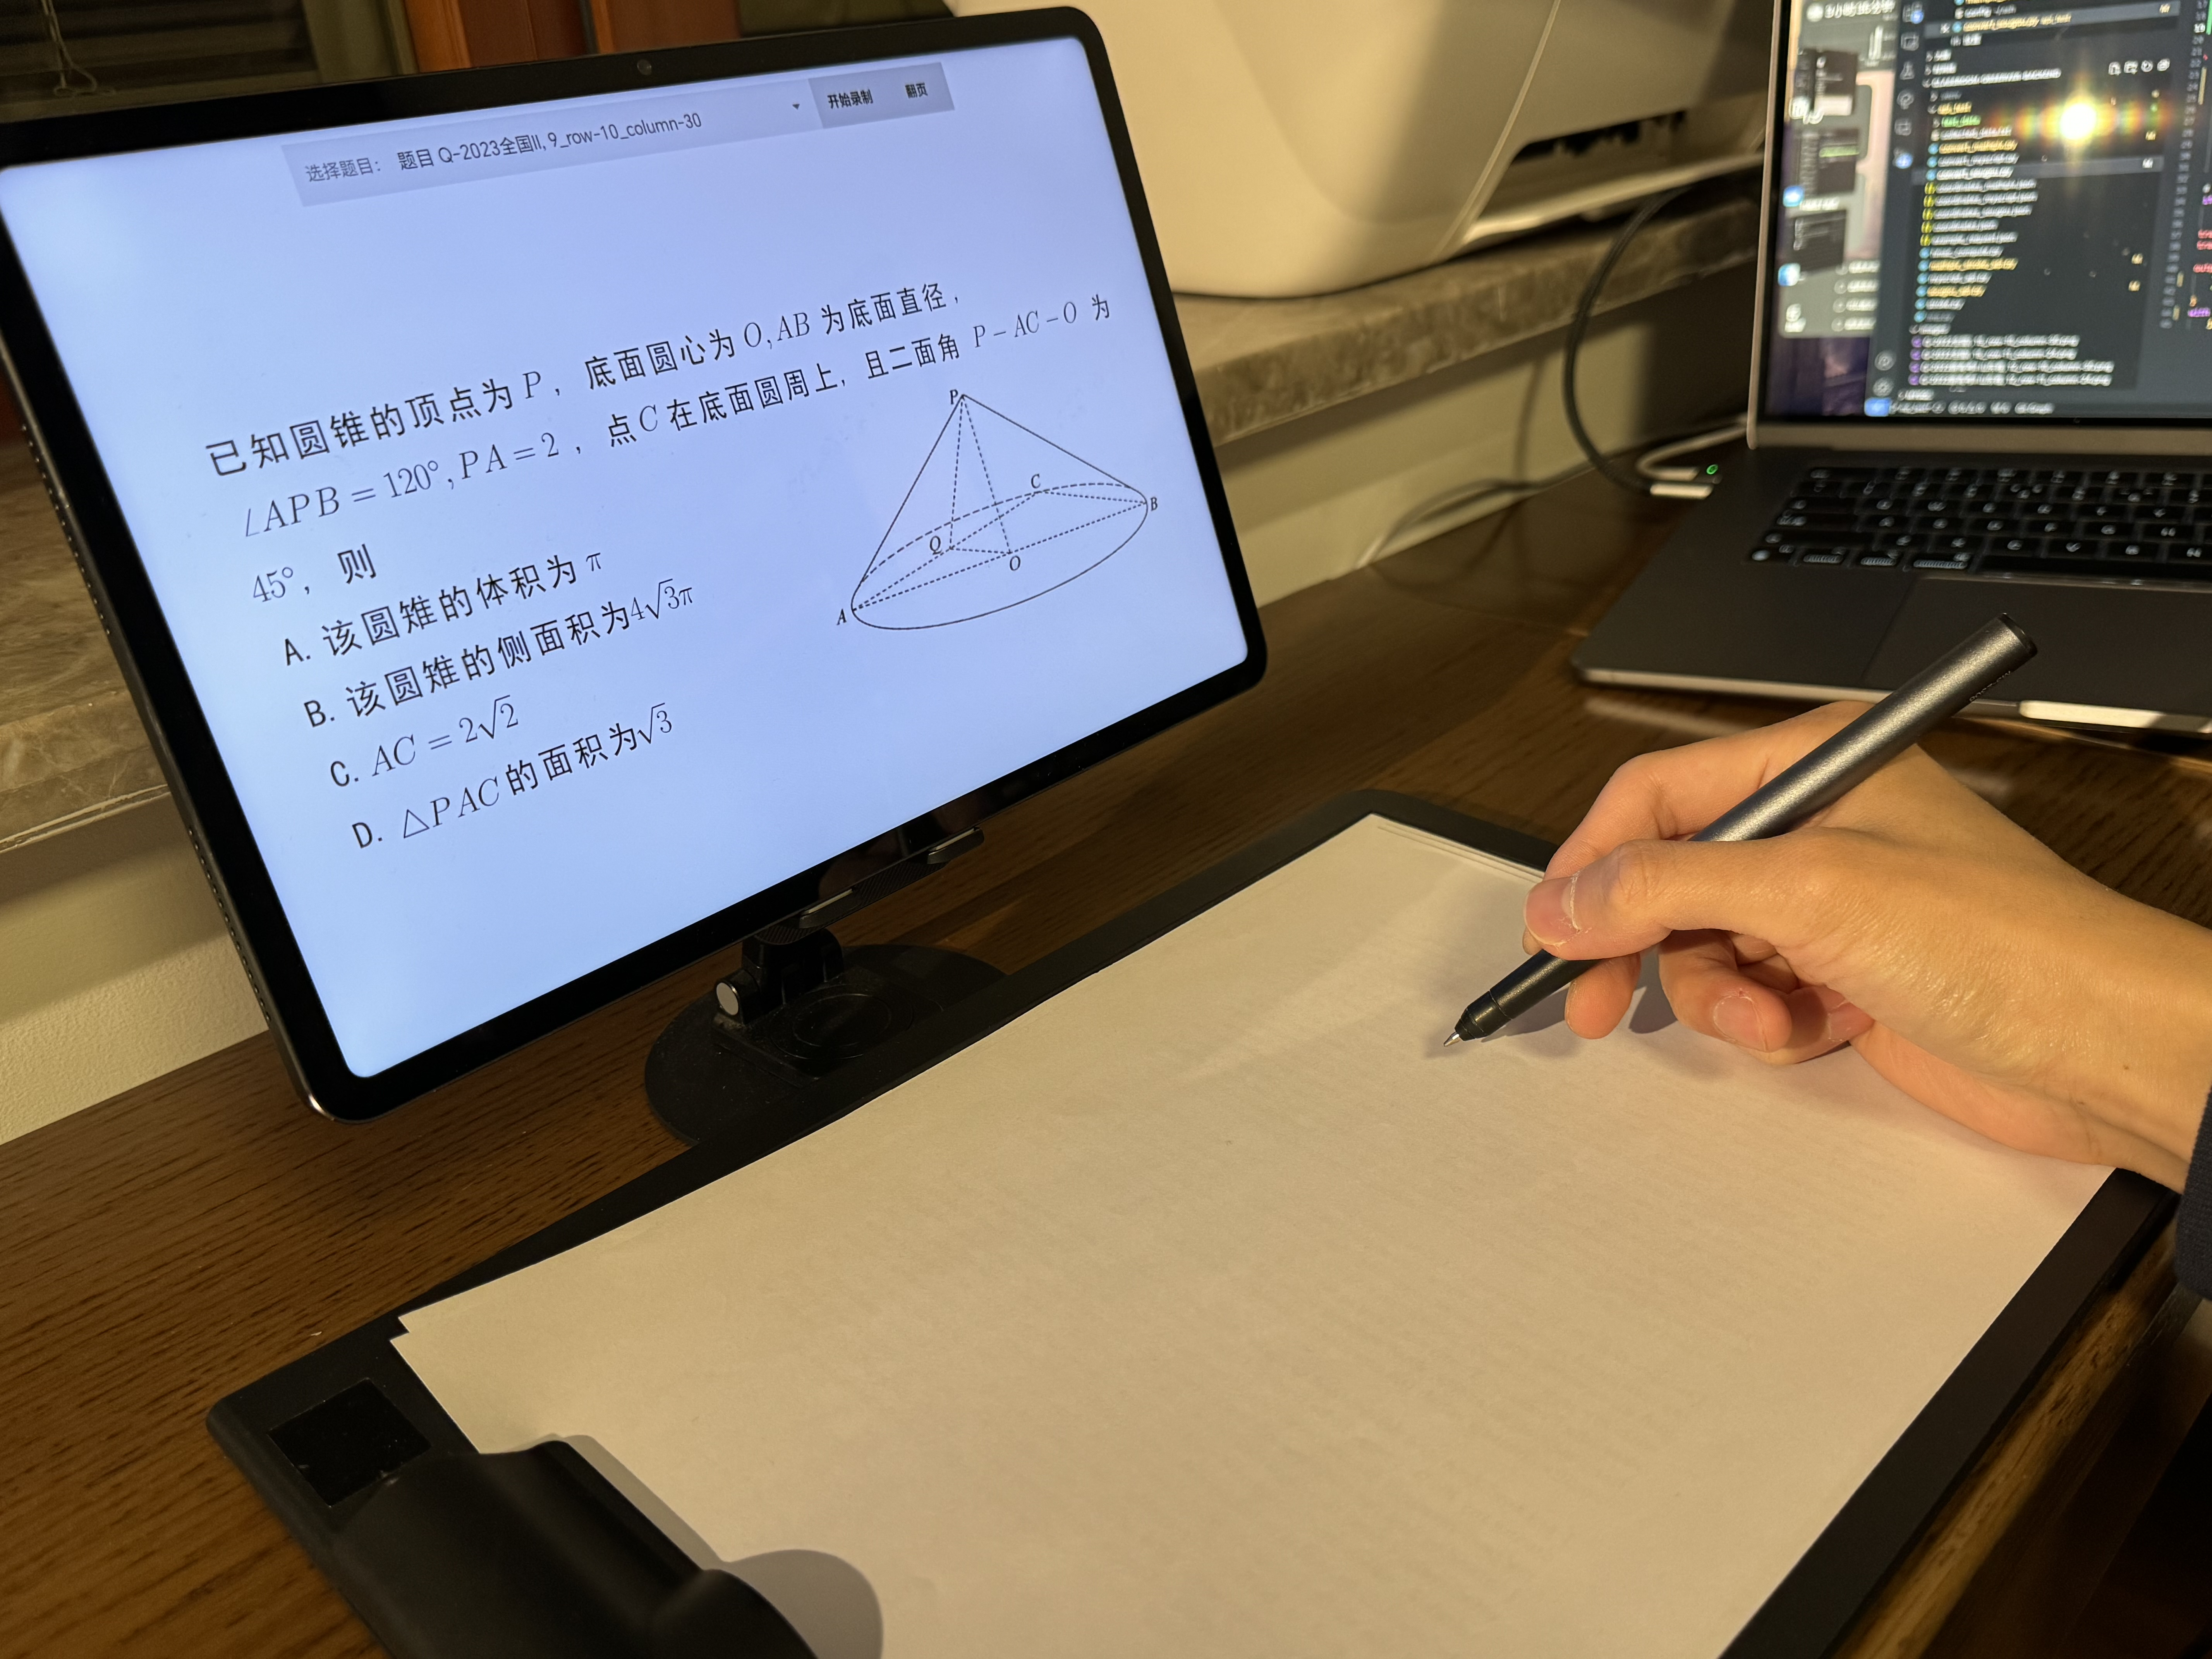
\includegraphics[width=0.7\linewidth]{experiment_setup.jpeg}
    \caption{实验设备}
    \label{fig:experiment_setup}
\end{figure}

\subsection{实验流程}

实验过程中,我们首先向被试介绍实验背景:我们希望探究如何对学生的解题思路进行跟踪和建模,所以现在需要尽可能详细地记录学生解数学题的过程。这个过程需要采集被试解题过程中的笔迹信息、视频和音频信息,并征求被试同意。实验的任务就是请被试现场解答上一节所述的三道数学题,这三个题目会按随机顺序展示给被试。

为了保证采集数据的质量,我们首先向被试明确实验过程的要求:被试在做题的过程中需要尽可能边思考边说(也称作要求被试 think aloud),尽可能把解题过程中的真实想法和思路说出来,哪怕这些想法暂时不正确也没关系。我们为被试提供了两种可能的表述方式:

\begin{itemize}
    \item 对于严谨的数学推理,可以按照:从已知条件中的\textbf{哪几个},运用什么\textbf{原理/规律},可以得到哪些\textbf{新的已知信息} 的模式来表述。
    \item 对于选择解题策略或探索可能的思路时的表述,可以参考:如果要求 A 的话,首先我们需要知道 B;看到题目给了\textbf{某些信息} ,所以首先想到应该求 X。
\end{itemize}

我们向被试强调,最重要的是被试需要尽量忠实地反映其思考过程,尽量自然地表述。不必局限于上述表达方式,用被试自己的话表达清楚就可以。

每道题开始前被试有最多 5 分钟的时间来读题和思考,如果有需要回忆具体的知识点的话,实验人员会提供必要的提示。之后正常解题,书写的内容包括草稿和解答都需要写在同一张纸上,由于采集笔迹设备的限制,书写不能超过一页 A4 纸。书写尽量顺序进行,从上到下。每道题完成后如果被试有思路表述不清楚的地方,可能会进行简单访谈。

\subsection{实验结果}

实验结束后,我们对实验数据进行了整理和分析。我们首先对实验数据进行了初步的整理,包括对笔迹数据的处理、视频和音频数据的提取,以及对实验过程中的访谈内容的整理。通过对本次实验所收集到的真实人类学生做题过程数据进行分析,我们总结了学生在解题过程中的表述特点,在表\ref{tab:biaoshutedian}中进行了概述。这些特点使得机器在理解学生的解题过程时面临一定的挑战,本节主要从解题思路刻画和语义理解这两个角度来分析。

\begin{table}
    \centering
    \caption{学生对解题过程的表述特点}
    \begin{tabular}{p{0.25\linewidth}p{0.75\linewidth}}
      \toprule
      \textbf{特点}             & \textbf{示例}                        \\
      \midrule
      一题多解         & 数列题目中的条件($\left\{\frac{S_n}{n}\right\}$ 为等差数列)翻译成数学语言,可以是 $\frac{S_n}{n} = cn+d$,也可以是 $\frac{S_{n+1}}{n+1} - \frac{S_n}{n} = c$,两种方法都能正确解答。 \\
      思路切换         & 对于数列题目,学生科能最初认为乙条件可以推出甲条件,但在观察后认为并不能,于是放弃了之前的思路,转而试图论证新的这一想法。                     \\
      跳步与解题顺序问题 & 对于选择题,不同被试会按不同的顺序来判断每个选项正误。    \\
      推理步骤表达上的模糊性 & 例如“……这个二面角是45度,因为是二面角所以PO等于QO”这一表述中,“这个二面角”并未指明是哪个二面角,需要结合学生所说的上下文以及题目信息来判断;而“因为是二面角所以PO等于QO”也并未讲清推理的详细依据。    \\
      推理步骤要素的缺失 & 学生在书写以及正常口语化表达的时候经常忽略“推导所依据的信息集合、推导使用的数学定律、以及得出的结果”这些要素中的一个或多个。    \\
      \bottomrule
    \end{tabular}
    \label{tab:biaoshutedian}
  \end{table}

所谓解题思路刻画,就是从宏观的视角,如何描述学生对于解题方法路径的选择,以及在不同的思路之间切换的问题。这方面主要有如下几个挑战:

\textbf{一题多解}:一道题目的求解往往可以有多种解法,尤其对于数学解答题。不同的解法可能从最开始的思路就不同,也可能在中途的某一部分采取了不同的路径。在实验中,我们发现被试对三道题的解答都有不止一种方法,其中的差别或多或少。这一特点这就给机器在理解学生解题过程时带来了一定的挑战,在判断解题正误的时候不能只对着一份标准解题过程判断,而是要在理解学生采取的方法的基础上去判断。对于我们的思维建模方法,也要能够支持多种解法的建模。

\begin{description}
    \item[例子] 对于数列那道题目,条件乙($\left\{\frac{S_n}{n}\right\}$ 为等差数列)的翻译可以有多种方式。比如有的被试将它翻译成 $\frac{S_n}{n} = cn+d$,有的被试则翻译成 $\frac{S_{n+1}}{n+1} - \frac{S_n}{n} = c$。这两种翻译方式对应的后续的推理过程不同,是不同的两种方法,但最终都能够求得正确结果。
\end{description}

\textbf{思路切换}:在解题过程中,学生可能会在某一步推理中遇到困难,或者发现了新的思路,从而选择放弃之前的思路,转而采取新的方法。这种思路切换可能会发生在任何一步,也可能会发生多次。这种思路切换也反映了学生的思维能力。我们的思维建模方法既需要能够记录下学生在不同思路之间尝试的过程,也需要能在这种情况下判断学生解题的正确性,进行准确的错因分析。

\begin{description}
    \item[例子] 数列题目的解答,有被试最初认为乙条件可以推出甲条件,但在观察后认为并不能,于是放弃了之前的思路,转而试图论证新的这一想法。这种表述类似于:“……然后证乙推出甲,因为等差数列求和公式一定要满足那个公式的样子,但是……诶?要考虑一下……好像刚才想得不太对,直觉上说乙应该不能推出甲。然后如果要验证一下的话,也许可以这样……”
\end{description}

\textbf{跳步与解题顺序问题}:即使采用了完全相同的解题思路,在解题过程的细节上仍然可能存在不同。比如有的被试可能会在某一步推理中跳过一些细节,直接给出结论,而有的被试可能会逐步展开推理过程。解题过程中的中间结果也可能以不同的顺序出现,比如一道题最终结论需要依赖A, B两个中间结论,有人可能会先得到A再得到B,也有人可能会先求得B再得到A,虽然这一顺序并不影响最终结果的得出,但表面上看却是两种解法。这就要求系统既能在详细刻画解题过程时区别二者,但在判断解题正确性时又不能因为这种细节上的差异而判断错误。

\begin{description}
    \item[例子] 对于立体几何选择题,不同被试会按不同的顺序来判断每个选项正误,尤其是被试先根据按照已知信息先把能够推理得到的信息都推出来再看选项的话,这种情况更容易出现。
\end{description}

另一方面,语义理解方面的挑战则是从微观的角度,能否通过学生对于每一步推理的表述,准确理解学生所想。这方面主要有如下几个挑战:

\textbf{推理步骤表达上的模糊性}:学生可能在表达特定的推理过程中使用使用模糊的用词来表达概念,仅仅根据这些描述和学生手写内容往往难以准确理解并转换成机器所能理解的结构化表达。在实验过程中,实验人员需要充分理解学生表述过程的语境与上下文,来推断模糊表述所对应的具体含义。这意味着我们的系统也需要较强的语义理解能力和上下文关联能力,才能准确地理解学生的表述。

\begin{description}
    \item[例子] 在解答解析几何题目时,有被试在描述步骤中使用了模糊的表达,例如:“……这个二面角是45度,因为是二面角所以PO等于QO”在这个表述中,“这个二面角”并未指明是哪个二面角,需要结合学生所说的上下文以及题目信息来判断;而“因为是二面角所以PO等于QO”也并未讲清推理的详细依据。
\end{description}

\textbf{推理步骤要素的缺失}:根据上文讨论,每一步推理从表述的完整性和严谨性上考虑,都需要包含推导所依据的信息集合、推导使用的数学定律、以及得出的结果。但是学生在书写以及口语化表达的时候经常忽略这些要素中的一个或多个。当然这一特点是正常语言表述习惯使然,但如果我们系统需要把学生的解题过程转化为结构化的数据,就需要解决这一问题,推断出学生表达中所缺失的部分。

\begin{description}
    \item[例子] 在解答导数题目时,有被试表述:“分析单调性的话先求导,求出来f(x)的导数是……”,这一表达实际就省略了求导的数学依据(f(x)中所包含的各个初等函数的导数公式)。
\end{description}

综合考虑学生在书写解答以及口头表述时的这些特点,我们提出一套学生解题思路建模方法,用来刻画学生的思维路径,位后续的系统设计奠定基础。

\section{学生思路建模方案}

本研究的目标是构建一个通过对学生解题思维的自动化建模和评估,进行自动化作业批改、错误定位、错因分析、知识点梳理等具体应用功能的智能系统。为了达成这一目标,我们首先需要一个能够准确地对学生解题思路进行建模的方法。这种对于思路的刻画方法需要具备以下特点:

\begin{itemize}
    \item \textbf{易于自动生成的}:我们的系统最终需要自动化地基于学生的表述来生成思路的表示,并在此基础上进行分析。
    \item \textbf{能够有效记录推理细节},包括推理的依据、使用的数学定律、以及得出的结论。
    \item \textbf{易于对比的}:我们需要能够比较不同学生的解题思路,以及学生的解题思路和标准答案之间的差异。
\end{itemize}

为了达到这一目标,我们提出了一套学生思维建模方案,对于学生的解题过程,我们使用两部分来表示:思维图和计算图。

\subsection{思维图}

对于学生思维的刻画,我们额外引入一个概念叫做\textbf{意图}(Intent)。对于解答过程,每一步进行了什么推导以及推导结果固然重要,但更重要的是学生是如何想到后续推理应当以什么为目标的。这一更高层面的信息更加能够反映学生的能力。因此,我们引入了意图的概念,用来表示学生在解题过程中某一时刻下的目标。此处所谓的思维图,就是以意图为核心的一系列表示,用来表示学生解题过程中的思维路径。图\ref{fig:siwei_graph}展示了一个思维图的例子,接下来会对这一例子进行详细说明。

\begin{figure}
    \centering
    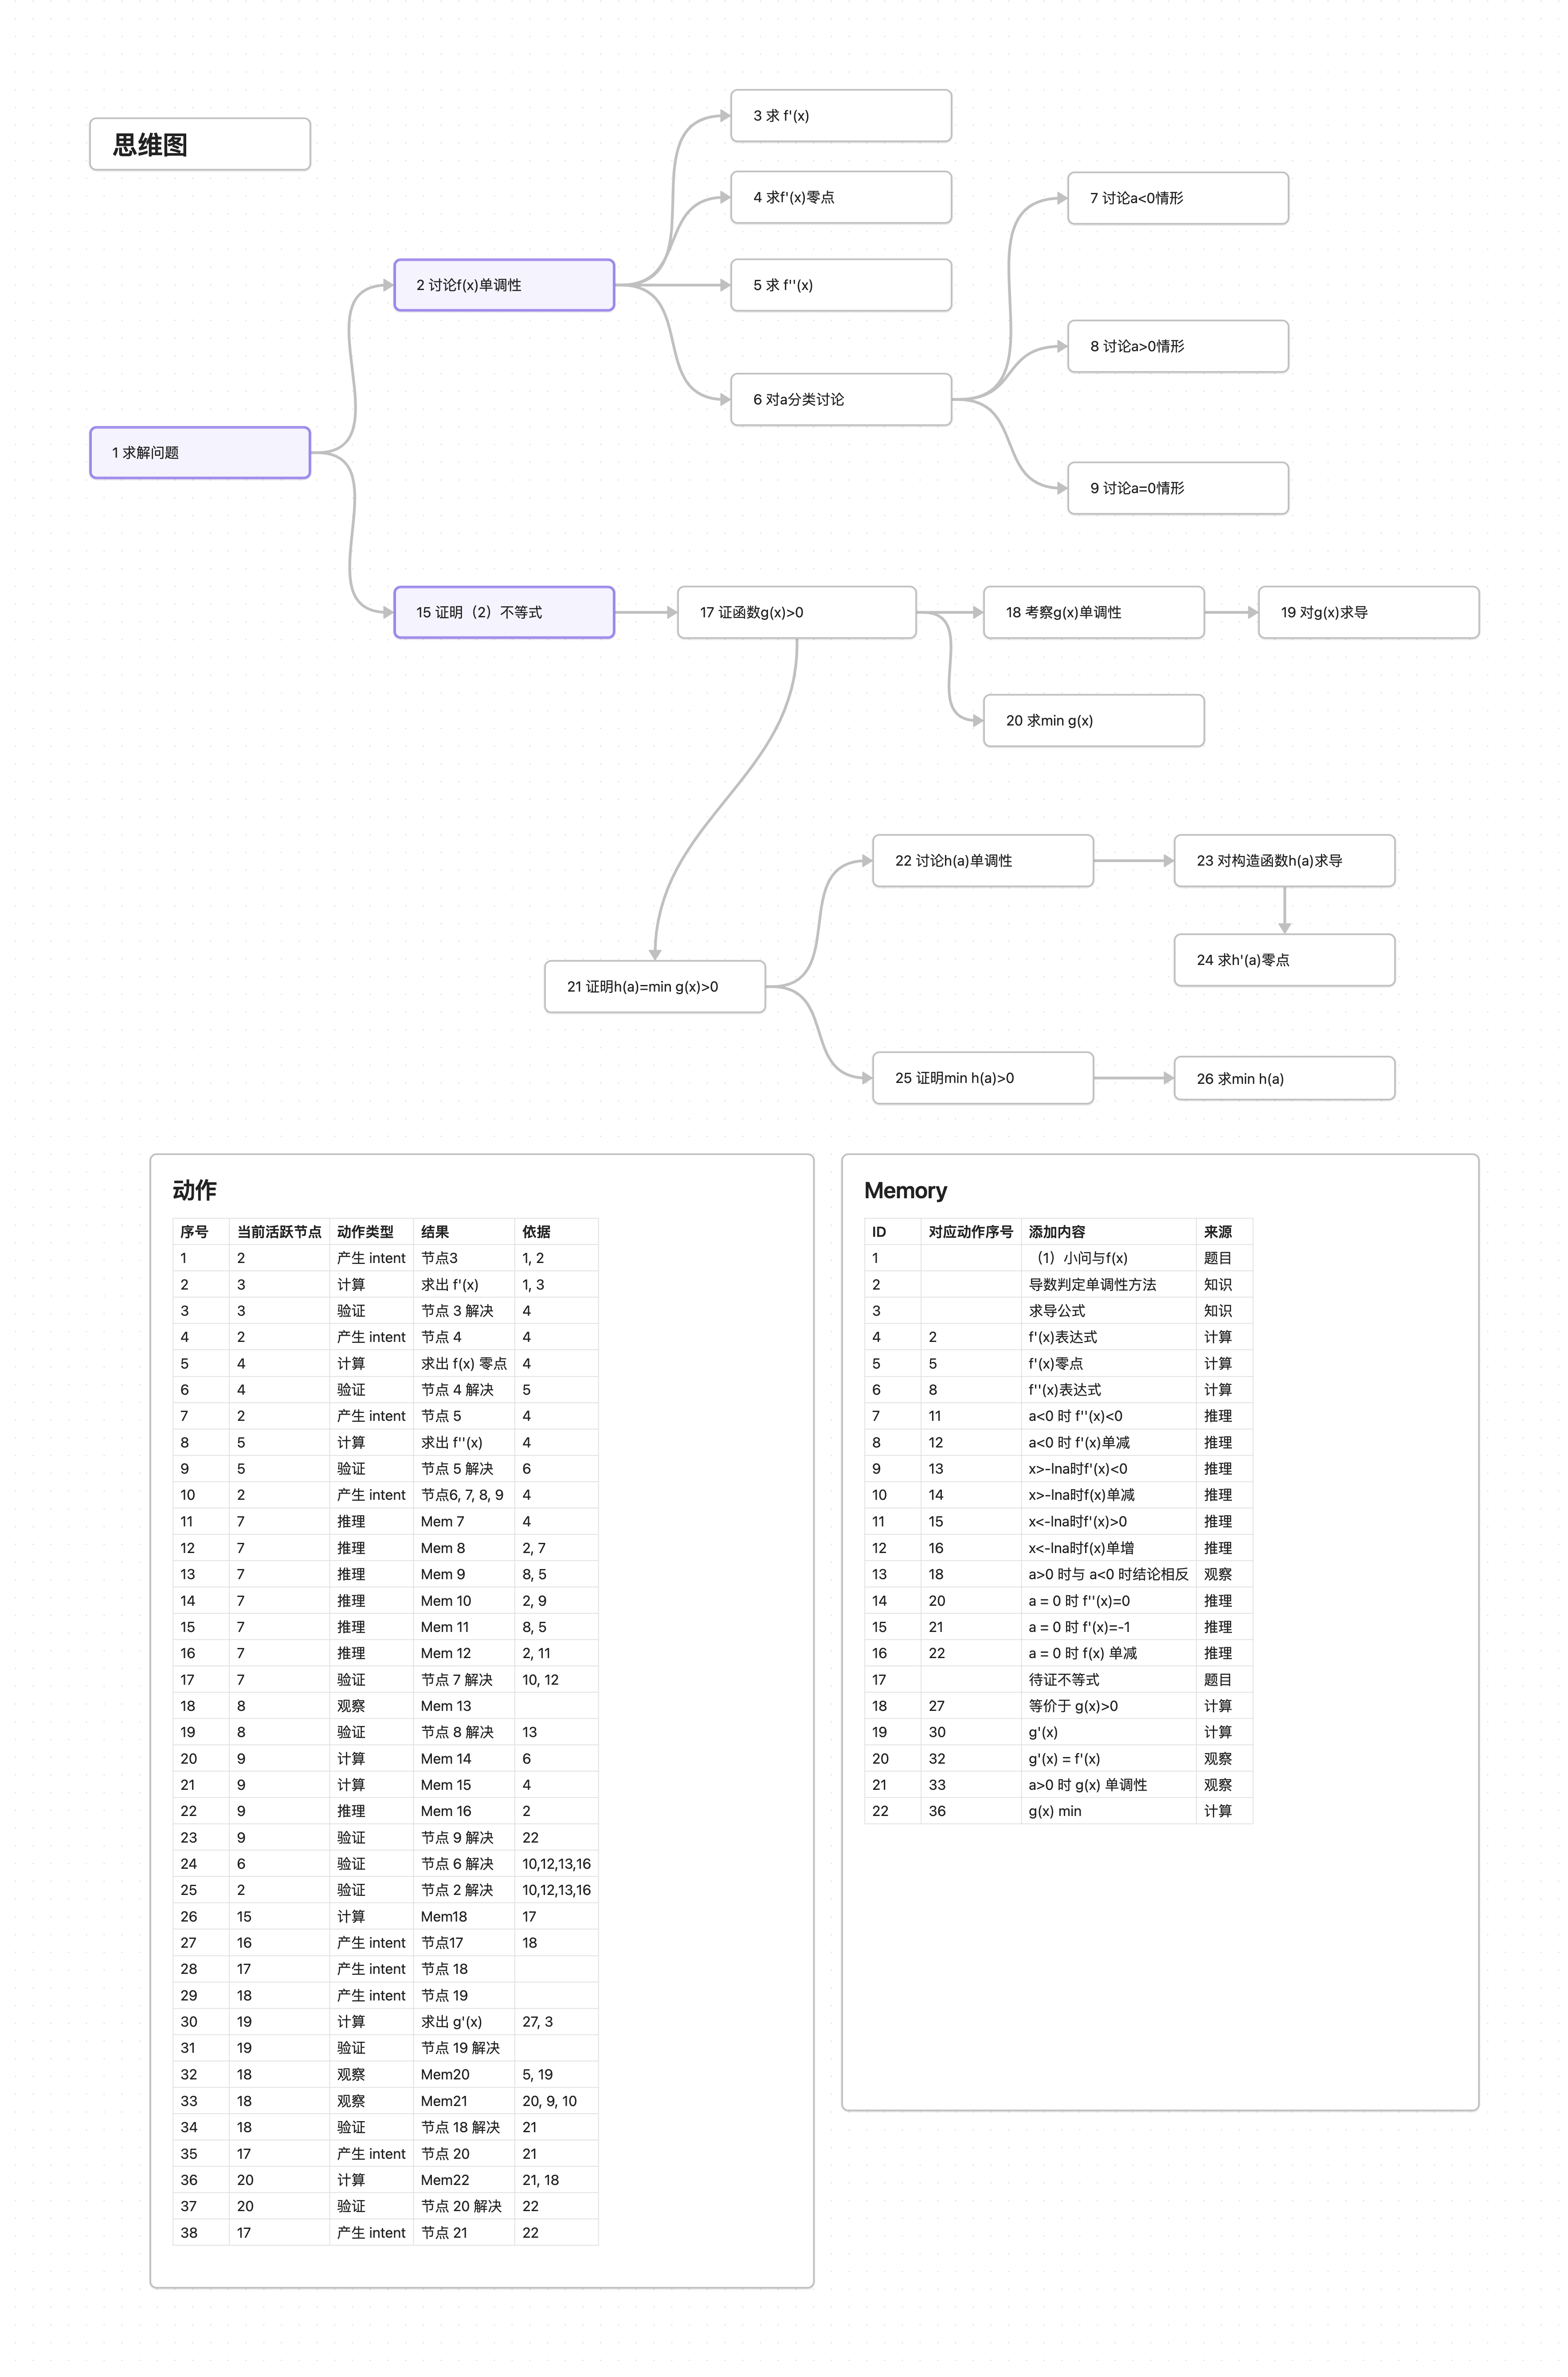
\includegraphics[width=\linewidth]{siwei_graph.png}
    \caption{基于前文所述导数题所作的思维图示例}
    \label{fig:siwei_graph}
\end{figure}

\subsubsection*{思维图的图结构}

在解题过程中,我们认为学生脑中的意图的动态类似一个栈。以图\ref{fig:siwei_graph}所示思维图为例,按照题目要求最初的意图是“讨论f(x)的单调性”,所以这一意图入栈,位于栈的最底部。根据常见的方法,分析单调性先求导,所以产生了下一个意图“求f'(x)”并入栈。接下来进行一系列计算,求得导数后栈顶的“求f'(x)”这一意图就被解决了,出栈。接着产生下一个意图并入栈,根据新的意图指导进行下一步的推理,新的意图也被解决之后出栈。经过一系列的推理过后,已有信息足以解决“讨论f(x)的单调性”这一意图,这一意图也最终被解决,“讨论f(x)的单调性”出栈。

思维图的图结构就是用来表示这一过程的,图中的每一个节点表示一个意图,节点的id表示了这些意图产生的时间顺序。每一条边表示意图之间的依赖关系:只有当一个意图的所有子节点都被解决,这个意图才能够被解决。图中的蓝色节点是题目的问题对应的意图,其他节点代表学生解题过程中出现的意图。

\subsubsection*{动作列表}

\subsubsection*{Memory}